\documentclass[oneside,14pt]{book}

\usepackage[T1,T2A]{fontenc}
\usepackage[utf8]{inputenc}
\usepackage[english,russian]{babel}
\usepackage{indentfirst}

%\usepackage[paperwidth=15cm,paperheight=7.5cm]{geometry} % планшет
%\usepackage[paperwidth=297mm,paperheight=210mm]{geometry} % A4
%\usepackage[paperwidth=148mm,paperheight=105mm]{geometry} % A5
\usepackage[paperwidth=18cm,paperheight=13cm,margin=5mm]{geometry} % экран*2

%\usepackage[colorlinks=true,
%]{hyperref}
%\newcommand{\email}[2]{#1\ \href{mailto:#2}{<\nolinkurl{#2}>}}
% %\newcommand{\email}[2]{\emph{#1\ <#2>}}
\usepackage[unicode,colorlinks,
pdftitle={Azbuka ARMaturschika (ru)},
pdfauthor={(c) Dmitry Ponyatov <dponyatov@gmail.com>, SSAU ASCL},
pdfsubject={ru manual on writing programs for Cortex-M MCUs},
pdfkeywords={ARM} {Cortex} {MCU} {ARMatura} {Arduino} {SSAU}
]{hyperref}

\usepackage{wrapfig}
\usepackage{graphicx}
\usepackage{epstopdf}
\DeclareGraphicsExtensions{.eps}

\usepackage{listings}
\usepackage{dirtree}
\usepackage[usenames,dvipsnames,svgnames]{xcolor}
\newcommand{\cppcolor}{\color[rgb]{0.94, 0.97, 1.0}} % Alice blue
\newcommand{\asmcolor}{\color[rgb]{0.98, 0.92, 0.84}} % Antique white
\newcommand{\ldcolor}{\color[rgb]{0.67, 0.9, 0.93}} % Blizzard Blue
\newcommand{\concolor}{\color[rgb]{0.88, 1.0, 1.0}} % Light cyan
\newcommand{\makecolor}{\color[rgb]{0.9, 0.9, 0.98}} % Lavender mist

%\definecolor{cppcolor}{rgb}{0.94, 0.97, 1.0}
\lstset{frame=single,
numbers=left, numberstyle=\small, numbersep=1mm,
tabsize=4,
keywordstyle=\color{blue}\texttt,
commentstyle=\color{cyan}\texttt,
inputencoding=utf8, extendedchars=true, showspaces=false,  
inputencoding=cp1251
}
\usepackage{lstlangarm}
\usepackage{lstlanggnumake}
\usepackage{lstlanggnuld}
\usepackage{lstlanggnudump}

\lstdefinestyle{cpp}{language=C++,backgroundcolor=\cppcolor}
\lstdefinestyle{asm}{language={[ARM]Assembler},backgroundcolor=\asmcolor}
\lstdefinestyle{gnuld}{language={[GNU]Link},backgroundcolor=\ldcolor}
\lstdefinestyle{con}{backgroundcolor=\concolor}
\lstdefinestyle{mk}{language=[GNU]Make,backgroundcolor=\makecolor}
\lstdefinestyle{objdump}{language=[GNU]Dump}

\newcommand{\cm}[1]{Cortex-M#1}
\newcommand{\cx}{\cm{x}}

\newcommand{\vld}{STM32VLDISCOVERY}

%\renewcommand{\url}[1]{\textbf{#1}}
\newcommand{\email}[1]{$<$\href{mailto:#1}{\textbf{#1}}$>$}

\newcommand{\cpp}{$C^{+^{+}}$}

\newcommand{\cp}[1]{\footnote{копипаста: #1}}

\newcommand{\thmod}{Thumb}
\newcommand{\armod}{ARM}
\newcommand{\arm}{ARM}

\newcommand{\Reg}[1]{\textbf{#1}}
\newcommand{\R}[1]{\Reg{R#1}}

\newcommand{\periph}[1]{\texttt{#1}}
\newcommand{\jtag}{\periph{JTAG}}

\usepackage{wasysym} % smileys
\usepackage{gensymb} % celsius
\usepackage{amssymb} % windows key
\usepackage{textcomp} % bigcircle

\usepackage[os=win]{menukeys}
\newcommand{\winstart}{$\boxplus$}
\newcommand{\file}[1]{\textbf{\textsf{#1}}}
\newcommand{\window}[1]{\textbf{\textit{#1}}}
\newcommand{\alarm}[1]{{\color{DarkRed}#1}}
\newcommand{\wcmd}[1]{\keys{\winstart+R}\ \directory{#1}}
\newcommand{\checkbox}{$\boxtimes$}
\newcommand{\uncheckbox}{$\square$}
\newcommand{\lms}{\keys{$\lhd$}}
\newcommand{\rms}{\keys{$\rhd$}}
\newcommand{\eclpx}{\window{Project Explorer}}

\newcommand{\win}[1]{
\includegraphics[height=10ex]{fig/winlogo.jpg} #1}
\newcommand{\lin}[1]{
\includegraphics[height=10ex]{fig/linuxcolor.png} #1}
\newcommand{\bug}{
\includegraphics[height=10ex]{fig/iconbug.png}}

\newcommand{\linux}{Linux}
\newcommand{\git}{Git}
\newcommand{\eclipse}{\textcircled{$\equiv$}\textsc{eclipse}}
%\newcommand{\term}[1]{\underline{#1}}
\newcommand{\term}[1]{\underline{\color{DarkBlue} #1}}
\newcommand{\miktex}{MiK\TeX}
\newcommand{\internet}{Internet}
\newcommand{\ql}{Quantum$^{\circledR}L^{e}aPs$}
\newcommand{\gdb}{GDB}

\newcommand{\make}{\file{make}}
\newcommand{\makefile}{\file{Makefile}}

\usepackage{tocloft}
\newcommand{\listlabname}{Лабораторные работы}
\newlistof{lab}{ex}{\listlabname}
\newcommand{\labpart}[1]{\addcontentsline{ex}{part}{#1}}
\newcounter{labworkcounter}
\newcommand{\labwork}[1]{
\refstepcounter{labworkcounter}
\section*{ЛР\thelabworkcounter: #1}
\addcontentsline{toc}{subsection}{ЛР\thelabworkcounter: #1}
\addcontentsline{ex}{section}{ЛР\thelabworkcounter: #1}
}
\newcommand{\labref}[1]{ЛР\ref{#1}}

\newcommand{\thetitle}{Азбука халтурщика-ARMатурщика}

\newcommand{\mytitle}[1]{
\title{\Huge{\thetitle}\\
#1\\
\normalsize{учебный курс по микроконтроллерам \cx:\\
Миландр 1986ВЕ, STM32F, LPC21xx}}
}

\author{(copypasta) Понятов Д.А. \email{dponyatov@gmail.com}, ИКП СГАУ}


\usepackage{tcolorbox}
\newcommand{\ru}[1]{{\color{blue}#1}}

\begin{document}
\mytitle{основы CMSIS}
\maketitle
\setcounter{tocdepth}{3}\tableofcontents

\section{\copyright}
\cp{двойной лось
\url{http://www.doulos.com/knowhow/arm/CMSIS/CMSIS\_Doulos\_Tutorial.pdf}}

\bigskip
This tutorial material is part of a series to be published progressively by
Doulos.

\bigskip
You can find the full set of currently published Tutorials and register for
notification of future additional at \url{www.doulos.com/knowhow}

\bigskip
You can also download the full source code of the examples used within the
Tutorial at the same URL.

\bigskip
Also check out the Doulos ARM Training and service options at
\url{www.doulos.com/arm}

\bigskip
Or email \email{info@doulos.com} for further information

\bigskip
First published by Doulos March 2009

\bigskip
Copyright 2009 Doulos. All rights reserved. All trademarks acknowledged. All
information is provided “as is” without warranty of any kind.

\section{Introduction}

The Cortex Microcontroller Software Interface Standard (CMSIS) supports
developers and vendors in creating reusable software components for 
\arm\ \cm{}\ based systems.

\ru{
Cortex Microcontroller Software Interface Standard (CMSIS)\footnote{стандарт
программного интерфейса микроконтроллеров Cortex}\ обеспечивает разработчикам и
производителям МК создание повторно используемых программных компонентов для
систем на основе микроконтроллеров \cm{}.
}

The \arm\ \cm{3}\ processor is the first core from ARM specifically designed for
the Microcontroller market. This core includes many common features (NVIC,
Timer, Debug-hardware) needed for this market. This will enable developers to
port and reuse software (e.g. a real time kernel) with much less effort to
\cm{3}\ based MCUs.

\ru{
Процессор \arm\ \cm{3}\ первое ядро от компании \arm\ специально разработанное
для рынка микроконтроллеров. Это ядро включает множество типовых блоков (NVIC,
таймеры, отладочный интрефейс) необходимых на этом рынке. Это позволяет
разработчикам с минимальными усилиями портировать и повторно использовать уже
написанное ПО\footnote{например ядро ОС реального времени}\ для МК семейства
\cm{3}\ любых производителей.
}

With a significant amount of hardware components being identical, a large
portion of the Hardware Abstraction Layer (HAL) can be identical. However,
reality has shown that lacking a common standard we find a variety of HAL/driver
libraries for different devices, which, as far as the \cm{3}\ part is
concerned essentially do the same thing\ --– just differently.

\ru{
Благодаря идентичности большого колиства аппаратных компонентов, также
идентичным оказывается и Hardware Abstraction Layer (HAL)\footnote{программный
слой аппаратной абстракции}.
Тем не менее, реальность показывает что отсутствие общего стандарта приводит к
множеству несовместимых версий библотек HAL и драйверов для различных МК, что не
соответствует идее полной переносимости ПО в серии \cm{3}.
}

The latest study of the development for the embedded market shows that software
complexity and cost will increase over time, see figure left.
Reusing Software and having a common standard to govern how to write and debug
the software will be essential to minimising costs for future developments.

\ru{
Последние исследования разработок для рынка встраиваемого ПО показывают, что
сложность программного обеспечения и его стоимость постоянно увеличиваются.
Повторное использование кода и наличие общего стандарта управляющего способами
написания и отладки ПО необходимы для минимизации стоимости разработки и
сопровождения.

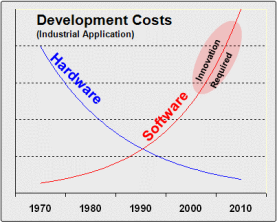
\includegraphics[height=30ex]{duolos_CMSIS/cmsisdevcosts.png}
стоимости разработки
}

\bigskip
With more \cm{3}\ based MCUs about to come onto the market, ARM has recognized
that after solving the diversity issue on the hardware side, there is still a
need to create a standard to access these hardware components.

\ru{
Анализируя ситуацию с взрывным ростом количества моделей МК \cm{3}\ на рынке,
компания \arm\ обнаружила что полная идентичность аппаратной части недостаточна
для обеспечения совместимости, и необходимо создание стандарта доступа к
аппаратным компонентам.
}

The result of that effort is CMSIS; a framework to be extended by vendors, while
taking advantage of a common API (Application Programming Interface) for core
specific components and conventions that define how the device specific portions
should be implemented to make developers feel right at home when they reuse code
or develop new code for ARM \cm{}\ based devices.

\ru{
Результатом этих исследований является \cmsis: фреймворк, расширямый
поставщиками МК, с сохранением полезных свойств общего API (Application
Programming Interface)\footnote{прикладной программный интерфейс} для ядреных
компонентов и соглашениями о том, как должны быть реализованы части зависимые от
железа, чтобы разработчики чувствовали себя как дома при повторном использовании
ил разработки нового кода для семейства \cm{}.
}

\section{Структура \cmsis}

CMSIS can be divided into three basic function layers:

\ru{\cmsis\ может быть поделен на три основных слоя:}

\begin{itemize}
\item Core Peripheral Access Layer (CPAL)

The lowest level defines addresses, and access methods for common components and
functionality that exists in every Cortex-M system. Access to core registers,
NVIC, debug subsystem is provided by this layer. Tool specific access to special
purpose registers (e.g. CONTROL, xPSR), will be provided in the form of inline
functions or compiler intrinsics. This layer will be provided by ARM.

\ru{
Самый нижний уровень определяет адреса, и методы доступа к общим компонентам и
функциям, существующим в каждой \cm{}-системе. Этим уровнем
описывается доступ к регистрам ядра, NVIC\footnote{Nested Vector Interrupt
Controller, контроллер вложенных прерываний}, подсистеме отладки.
Инструментальный доступ к спецрегистрам (\file{CONTROL},\file{xPSR})
предоставляется в форме inline-функций или интринсик компилятора. Этот уровень
обеспечивается лицензиатом архитектуры\ --- компанией \arm.
}

\item Middleware Access Layer (MWAL)

This layer is also defined by ARM, but will be adapted by silicon vendors for
their respective devices.
The Middleware Access Layer defines a common API for accessing peripherals. The
Middleware Access Layer is still under development and no further information is
available at this point.

\ru{
Этот слой также специфицируется \arm, но адаптируется производителем кристаллов
для их конкретных изделий. Слой MWAL определяет общий API для доступа к
периферии. Этот слой все еще находится на стадии доработки, и на текущий момент
более подробная информация неступна.
}

\item Device Peripheral Access Layer (DPAL)

Hardware register addresses and other definitions, as well as device specific
access functions will be defined in this layer. The Device Peripheral Access
Layer is very similar to the Core Peripheral Access Layer and will be provided
by the silicon vendor. Access methods provided by CPAL may be referenced and the
vector table will be adapted to include device specific exception handler
address.

\ru{
Слой содержит адреса аппаратных регистров и другие определения, в том числе
функции доступа к специфичным особенностям чипов.
DPAL сильно похож на CPAL, но предоставляется поставщиком кристаллов.
В CPAL могут быть описаны методы доступа и адаптированная таблица векторов,
содержащая обработчики исключений, специфичные для конкретного МК.
}

While DPAL is intended to be extended by the silicon vendor, let’s not forget
about Cortex-M based FPGA products, which effectively put developers into the
position of a silicon vendor.

\ru{
DPAL предназначен для расширения вендором, но не стоит забывать о
FPGA-продуктах с примением \cm{}-ядер, которые ставят разработчиков в положение
вендора.
}

\end{itemize}

The basic structure and the functional flow is illustrated in the Figure 2. below.

\bigskip
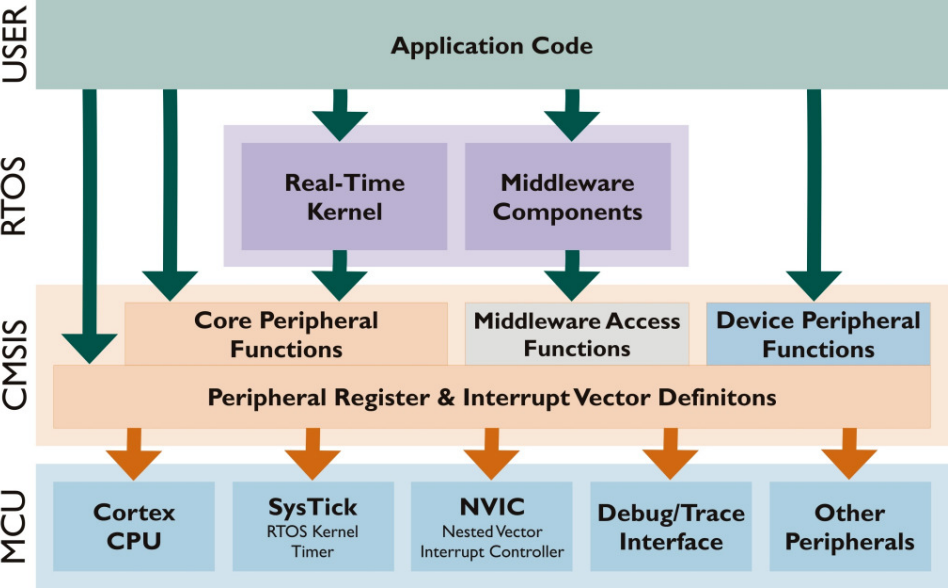
\includegraphics[width=0.9\textwidth]{duolos_CMSIS/cmsisstruc.png}

Figure 2 CMSIS Structure functional flow

\ru{Рис.2 Функциональная структура CMSIS}

\bigskip
As far as MCU based systems are concerned it might make sense for developers to
treat the entire PCB system as monolithic block. There is no reason to
differentiate between a memory mapped register inside the MCU and a memory
mapped register external to the MCU, connected via external memory interface.
The benefit of applying a standard like CMSIS is that existing guidelines on how
to access these devices set a clear goal on how to implement and integrate
critical parts of the software.
Other team members will find a familiar environment.

\subsection{File Structure}

File names in CMSIS are standardized as follows:

\begin{tcolorbox}
\begin{tabular}{l l}
\file{core\_cm3.h} &\cm{3}\ global declarations and definitions, static
function definitions \\
\file{core\_cm3.c} &\cm{3}\ global definitions\\
\file{<device>.h} &Top-level header file (device specific). To be included by
application code.\\
&Includes \file{core\_cm3.h} and \file{system\_<device>.h}\\
\file{system\_<device>.h} &Device specific declarations\\
\file{system\_<device>.c} &Device specific definitions, e.g.
\verb|SystemInit()|\\
\end{tabular}
\end{tcolorbox}

Application code will only include the top-level header file which implicitly
pulls in all other essential

\bigskip
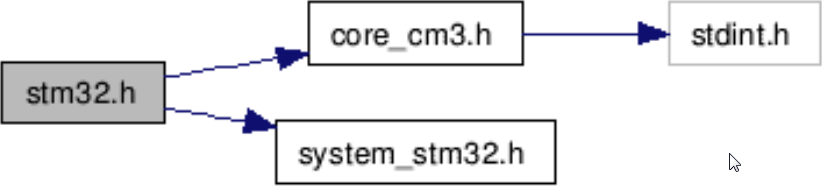
\includegraphics[width=0.5\textwidth]{duolos_CMSIS/stm32.png}
\bigskip

header files. The illustration below shows the flow and dependencies of the
header files \file{stm32.h}, \file{core\_cm3.h} and \file{system\_stm32.h},
which are part of CMSIS release V1P0.

\begin{lstlisting}[style=cpp]
/* Configuration of the Cortex-M3 Processor and Core Peripherals */
#define __MPU_PRESENT 0			 /*!< STM32 does not provide a MPU present or not*/
#define __NVIC_PRIO_BITS 4		 /*!< STM32 uses 4 Bits for the Priority Levels */
#define __Vendor_SysTickConfig 0 /*!< Set to 1 if different SysTick Config isused */
 
#include "core_cm3.h" 	 		 /* Cortex-M3 processor and core peripherals */ 
#include "system_stm32.h" 		 /* STM32 System */
\end{lstlisting}

The \file{<device>.h} file is the central include file and provided by the
silicon vendor. The application programmer is using that as the main include file in his
C source code. Note that the ARM \cm{3}\ has some optional hardware features
(e.g. the MPU, number of Interrupts and the number of the NVIC priority bits)
the silicon vendors may have implemented differently. The listing above shows
that STM32 implements four out of eight possible priority bits. The macro
\verb"__NVIC_PRIO_BITS"\ is set here to 4. STM32 does not offer a Memory
Protection Unit (MPU). Accordingly, the macro \verb"__MPU_PRESENT"\ has the
value 0.

The next example shows the corresponding definitions for a NXP LPC17xx device.
In this Cortex-M3 implementation five priority bits have been implemented and an
MPU is available.

\begin{lstlisting}[style=cpp]
/* Configuration of the Cortex-M3 Processor and Core Peripherals */
#define __MPU_PRESENT 1 		 /*!< MPU present or not */
#define __NVIC_PRIO_BITS 5 		 /*!< Number of Bits used for Priority Levels */
#define __Vendor_SysTickConfig 0 /*!< Set to 1 if different SysTick Config is used */

#include "..\core_cm3.h" 	/* Cortex-M3 processor and core peripherals */
#include "system_LPC17xx.h" /* System Header */
\end{lstlisting}

The \verb"__Vendor_SysTickConfig"\ defined is showing in both cases the default
setting. When this macro is set to 1, the \verb|SysTickConfig()|\ function in
the \file{cm3\_core.h}\ is excluded. In this case the file 
\file{<device>.h}\ must contain a vendor specific implementation of this
function.

\subsection{Tool Independence}

CMSIS exists in a three-dimensional space of the form
vendor$\div$device$\div$tool chain.
In order to remove one dimension (tool chain), the common files
\file{core\_cm3.c}\ and \file{core\_cm3.h}\ contain all essential tool specific
declarations and definitions.

\bigskip
Example:

\begin{lstlisting}[style=cpp]
/* define compiler specific symbols */
#if defined ( __CC_ARM )
	#define __ASM __asm				/*!< asm keyword for armcc */
	#define __INLINE __inline		/*!< inline keyword for armcc */
#elif defined ( __ICCARM__ )
	#define __ASM __asm				/*!< asm keyword for iarcc */
	#define __INLINE inline			/*!< inline keyword for iarcc.
									Only avaiable in High optimization mode! */
	#define __nop __no_operation	/*!< no operation intrinsic in iarcc */
#elif defined ( __GNUC__ )
	#define __ASM asm 				/*!< asm keyword for gcc */
	#define __INLINE inline 		/*!< inline keyword for gcc */
#endif
\end{lstlisting}

The remaining parts of CMSIS can now simply use the macro \verb|__INLINE|\ to
define an inline function.

\ru{Остальная часть \cmsis\ теперь может просто использовать макрос}
\verb|__INLINE|\ \ru{для определения инлайн-функций.}

\bigskip
Currently three of the most important C-compilers are supported: ARM RealView
(armcc), IAR EWARM (iccarm), and GNU Compiler Collection (gcc). This is expected
to cover the majority of tool chains.

\ru{
На настоящий момент поддерживаются три наиболее применяемых Си-компилятора:
ARM RealView (armcc), IAR EWARM (iccarm), и GNU Compiler Collection (gcc).
}

\subsection{MISRA-C}

Besides defining an API for Cortex-M core peripherals and guidelines on how to
support device peripherals, CMSIS defines some coding guidelines and
conventions. Most important is that the CMSIS code base is MISRA-C 2004
compliant, which implies that every extension should be compliant, too. MISRA-C
is a set of safety rules established by the “Motor Industry Software Reliability
Association” for the C programming language. Maintaining MISRA compliance can be
tricky, in particular when implementing driver level software. Therefore,
pragma-like exceptions in PCLint style are scattered across the source code. Be
aware that other tools, e.g. MISRA checker in IAR EWARM, might flag errors. Each
exception is accompanied with a comment explaining why this exception was made.

\subsection{CPAL Functions}

All functions in the Core Peripheral Access Layer are reentrant and can be
called from different interrupt service routines (ISR). CPAL functions are also
non-blocking\footnote{Memory barriers are exempt from that rule although they
might stall the processor for a few cycles.}\ in the sense that they do not 
contain any wait-loops.

The majority of functions in the CPAL have been implemented in the header file
\file{core\_cm3.h}\ as \verb|static| \verb|inline| functions. This allows the
compiler to optimize the function calls by placing the instructions that make up the called
function along with other code from which the function was called.

\subsection{Interrupt Service Routines}

Exception handlers will get a name suffix \verb|_Handler|, while (external)
interrupt handlers get the suffix \verb|_IRQHandler|. There must be a default
handler for each interrupt, which executes an infinite loop.
Tool specific configuration must make sure that this default handler will be
used as fall-back if no user-provided handler exists. It done
Through \verb|__weak| declaration in EWARM and RVCT armcc,
\verb|__attribute__((weak))| in GCC and RVCT armcc and
\verb|[WEAK]| export in RVCT/armasm.

Given that the \cm{}\ NVIC provides byte-arrays and bit-strings to configure
priorities and interrupt source en-/disable, an enumerated type \verb|IRQn_t|
with an element for each exception/interrupt position with the suffix
\verb|_IRQn|\ must be defined for each interrupt (\file{<device>.h}). The system
handler names are common for all devices and must not be changed.

\begin{lstlisting}[style=cpp,title=Listing shows the generic part of the
(\file{<device>.h}) file.] typedef enum IRQn
{
/****** Cortex-M3 Processor Exceptions Numbers *******************************/
 NonMaskableInt_IRQn = -14, 	/*!< 2 Non Maskable Interrupt */
 MemoryManagement_IRQn = -12, 	/*!< 4 Cortex-M3 Memory Mgmt Interrupt */
 BusFault_IRQn = -11, 			/*!< 5 Cortex-M3 Bus Fault Interrupt */
 UsageFault_IRQn = -10, 		/*!< 6 Cortex-M3 Usage Fault Interrupt */
 SVCall_IRQn = -5, 				/*!< 11 Cortex-M3 SV Call Interrupt */
 DebugMonitor_IRQn = -4, 		/*!< 12 Cortex-M3 Debug Monitor Interrupt */
 PendSV_IRQn = -2, 				/*!< 14 Cortex-M3 Pend SV Interrupt */
 SysTick_IRQn = -1, 			/*!< 15 Cortex-M3 System Tick Interrupt */
/****** Device specific Interrupt Numbers ************************************/
 UART_IRQn = 0, 				/*!< Example Interrupt */
} IRQn_Type;
\end{lstlisting}

All system handlers have negative virtual slot numbers so that they can be
distinguished in functions that abstract from the differences between system
handlers and external interrupt handlers. External interrupt handlers start at
the index 0.

\subsection{Other Coding Conventions}

The CMSIS documentation recommends a few more things regarding capitalization of
identifiers, commenting code.

\subsubsection{Identifiers}

\begin{itemize}
  \item Capital names to identify Core Registers, Peripheral Registers, and CPU
  Instructions.
  
  E.g.: \verb|NVIC->AIRCR|, \verb|GPIOB|, \verb|LDMIAEQ|
  
  \item “CamelCase” (mix of upper- and lower-case letters) names to identify
  peripherals access functions and interrupts.

 E.g.: \verb|SysTickConfig()|, \verb|DebugMonitor_IRQn|

  \item Peripheral prefix (\verb|<name>_|) to identify functions that belong to
  specific peripherals.

 E.g.: \verb|ITM_SendChar()|, \verb|NVIC_SystemReset()|

\end{itemize}

\subsubsection{Comments}

CMSIS uses \term{Doxygen}\ style comments for all definitions and encourages
developers to do the same.

In particular, the comment for each function definition should at least contain

\begin{itemize}
\item one-line brief function overview. (Tag: \verb|@brief|)
\item detailed parameter explanation. (Tag: \verb|@param|)
\item detailed information about return values. (Tag: \verb|@return|)
\item detailed description of the actual function.
\end{itemize}

The example below shows the beginning of a function definition:

\begin{lstlisting}[style=cpp]
/**
 * @brief Enable Interrupt in NVIC Interrupt Controller
 *
 * @param IRQn_Type IRQn specifies the interrupt number
 * @return none
 *
 * Enable a device specific interupt in the NVIC interrupt controller.
 * The interrupt number cannot be a negative value.
 */
static __INLINE void NVIC_EnableIRQ(IRQn_Type IRQn)
{
// . . .
}
\end{lstlisting}

The tags can be parsed by the documentation tool Doxygen, which is used to
create cross-referenced source code documentation in various formats
(\url{http://www.stack.nl/~dimitri/doxygen/index.html}). The tag syntax is
rather minimalistic and does not impair readability of the source code. Please
consult the Doxygen Documentation for details about tag syntax.

As an alternative to regular C block comments (\verb|/* */|) CMSIS explicitly
allows line comments (\verb|//|, so called C++-comments). If you are concerned
about MISRA compliance, be aware though, that MISRA-C 2004 doesn’t allow line
comments according to rule 2.2.

\ru{
CMSIS предлагает альтернативу обычным сишным /* блочным комментариям */ в виде
// строчных комментариев, так называмых \cpp-комментариев. Если вас беспокоит
выполнение превил MISRA, учтите что} \alarm{MISRA-C:2004 не разрешает
использовать строчные комментарии согласно правилу 2.2}.

\subsubsection{Data Types}

All data types referenced by CMSIS are based on those defined in the standard C
header file \file{stdint.h}. Data structures for core registers are defined
CMSIS header file \file{core\_cm3.h}, along with macros for qualifying registers
according to their access permissions. The rationale is that tools might be able
to automatically extract that information for debug purposes.

\begin{lstlisting}[style=cpp]
#define 	__I 	volatile const	/*!< defines 'read only' permissions */
#define		__O 	volatile 		/*!< defines 'write only' permissions */
#define 	__IO 	volatile 		/*!< defines 'read / write' permissions */
\end{lstlisting}

\subsection{Debugging}

A common requirement in software development is some sort of terminal output for
debugging. Text/graphics displays in embedded devices cannot be assumed to be at
hand (or might be in use), which previously left the developer with essentially 
two choices:

\begin{enumerate}
\item Use one of the ubiquitous UARTs and connect a terminal

Issues: All UARTs might be in use, access to UART signals might not be possible
for reasons that include pin-sharing, PCB layout, etc.

\item Use the semihosting mechanism

Issue: Significant software overhead on target CPU, might not be supported in
the same way by all tool chains, potential impact on timing behavior.
\end{enumerate}

With \cm{3}\ the preferred method makes use of the Instrumentation Trace
Macrocell (ITM), which is part of the processor macro cell and thus always
present.\footnote{Always present in \cm{3}\ rev1 cores. \cm{3}\ rev2 makes
ITM an optional feature.}

A Serial Wire Viewer (SWV) capable debug adapter can receive ITM data through
the SWO (Serial Wire Out) debug pin. ITM implements 32 general purpose data
channels. CMSIS builds on top of this and declares channel 0 to be used for
terminal output, along with a function called \verb|ITM_SendChar()| which can be
used as low-level driver function for printf-style output. A second channel (31) 
has been reserved for OS aware debugging, which means that a kernel can use it
to transmit kernel specific data which could then be interpreted by the debug
tool. 

With this standardization, tool vendors have it much easier to implement
specific debug features, such as e.g. terminal emulation for data received via
ITM channel 0. Developers on the other hand can rely on this feature to dump
state information, without having to configure UARTs and external terminal
emulators. See our Tutorial 2 later in this document.

Access privilege can be configured for groups of ITM channels. In order to use
ITM channel 0, unprivileged access must be granted, whereas ITM channel 31 is in
a different group and may allow privileged access only.

\subsection{Future Updates}

The CMSIS developers have taken care to provide macros indicating the CMSIS
version used in a project. That way provisions can be made to prevent code to be
used with a different CMSIS version than originally intended.

\begin{lstlisting}[style=cpp]
#define __CM3_CMSIS_VERSION_MAIN (0x01)		/* [31:16] main version */
#define __CM3_CMSIS_VERSION_SUB (0x10)		/* [15:0] sub version */

#define __CM3_CMSIS_VERSION ((__CM3_CMSIS_VERSION_MAIN << 16) | \
							__CM3_CMSIS_VERSION_SUB)
\end{lstlisting}

\section{Tutorial 1 – A First Example}
\subsection{Example 1 Starting point}
\subsection{Example 2 Converting to CMSIS}
\section{Tutorial 2 – ITM Debug}
\section{Summary}

\addcontentsline{toc}{part}{Литература}
\begin{thebibliography}{9}

\bibitem{leaps}{\copyright\ Quantum Leaps}

\bibitem{milandr}{\url{http://milandr.ru/} ЗАО <<ПКК Миландр>>}

\bibitem{progit}{\url{http://git-scm.com/book/ru} перевод:
Scott Chacon
\textbf{Pro Git}
}

\bibitem{habraQP}{\url{http://habrahabr.ru/post/114239/} хабра: Quantum Leaps QP
и диаграммы состояний в UML}

\bibitem{quantumleaps}{\url{http://www.state-machine.com/}
Quantum$^{\circledR}L^{e}aPs$ State Machines \& Tools}

\end{thebibliography}

\end{document}
